\documentclass[11pt]{article}
\usepackage{graphicx}
\graphicspath{ {images/} }
\usepackage{geometry}
\geometry{a4paper}

\begin{document}

\section{15th of January 2015}
The project was introduced and the group was formed and we exchanged basic information about ourselves. We decided that we would use Java and discussed the time of next meeting. And decided that we would meet every Thursday at 10 o'clock.
\subsubsection{Members:}
\begin{itemize}
\item Balazs Kiss
\item Eddy Mukasa
\item Gabb Visessmit
\item Pongsakorn N. Riyamongkol
\item Snorri Hannesson
\end{itemize}
\newpage

\section{19th of January 2015}
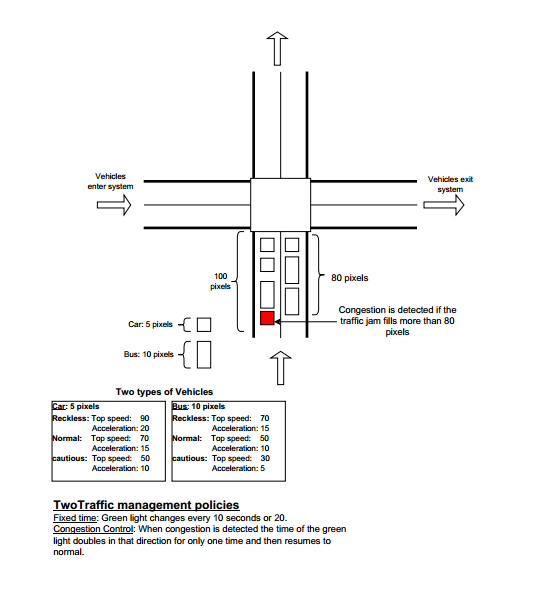
\includegraphics{meeting2}
\newpage

\section{21st of January 2015}
We discussed more technical aspects of the implementation; what classes we would create and their interrelation, what GUI platform we would use, how we would implement tests and when to start the test phase and if one of us should have the role of a tester, what IDE is nice, how Github works, ect. We decided that we would use a project management style built on iterations, start with building a simple prototype and try move closer towards the final product in each iteration. Finally we allocated work among ourselves unit next meeting:
\begin{itemize}
\item \textbf{Everyone:} Think about how to implement the project.

\item \textbf{Balazs:} Creating a project and making the first lines of code and put on Github.

\item \textbf{Eddy:} Creating a first draft of a UML diagram.

\item \textbf{Gabb and Neab:} Familiarise themselves with Github and GUI implementation with JavaFX.

\item \textbf{Snorri:} Write meeting log, and start the initial report.

\end{itemize} 

\newpage

\section{29th of January 2015}
\begin{itemize}
\item We discussed the the structure of the initial report and then revised the progress so far on the initial report. We discussed in particular what role each member should have, what project management style we should use and strategy.
\item We decided to use Trello for task management.
\item Roles: Balazs - (lead) programmer, Gabb - (lead) graphical designer, Eddy - (lead) software architect, Neab - Project manager and Snorri - (lead) tester. So each member would supervise his sector of the project; for instance Eddy could make some unit test bench but Snorri would oversee all the tests and make sure that everything would be tested, etc.
\item We discussed some branching strategies on github. 
\end{itemize} 

\newpage


\end{document}